\documentclass{beamer}

\usepackage[utf8]{inputenc}
\usepackage{default}
\usepackage[absolute,overlay]{textpos} % positioning the block in every where with a coordinate
% 
% foot citation
\usepackage{biblatex}
\bibliography{mi_ref}

\newcommand{\semfootnote}[1]{\let\thefootnote\relax\footnotetext{#1}}

% \usepackage{graphicx}
\usepackage{caption}
\usepackage{subcaption}

\usepackage{tikz}
\usetikzlibrary{arrows,shapes}

\tikzset{
  every overlay node/.style={
    %draw=black,fill=white,rounded corners,
    anchor=north west, inner sep=0pt,
  },
}
% Usage:
% \tikzoverlay at (-1cm,-5cm) {content};
% or
% \tikzoverlay[text width=5cm] at (-1cm,-5cm) {content};

% \def\tikzoverlay{%
%    \tikz[remember picture, overlay]\node[every overlay node]
% }%

 \usetheme{Tpt}
\begin{document}
\tikzstyle{every picture}+=[remember picture]

% By default all math in TikZ nodes are set in inline mode. Change this to
% displaystyle so that we don't get small fractions.
\everymath{\displaystyle}

\title[High level image understanding using logical and morphological approaches]{Mid-term Evaluation \\ High level image understanding using logical and morphological approaches}
\author[Yifan YANG]{\begin{tabular}{r@{ }l} 
     Yifan & YANG \\[1ex] 
Advisors: & Isabelle BLOCH\\
             & Jamal ATIF
\end{tabular}}
\institute{Telecom ParisTech}
% \date{\today}
\date{March 30, 2015}
%====================Title Page=================================
\begin{frame}[plain]
\titlepage
\begin{textblock}{100}(33,80)
     
\includegraphics[height=1cm,width=1cm]{images/telecom.png}
     
\includegraphics[height=1cm,width=1.2cm]{images/logocnrs.png}
     
\includegraphics[height=1cm,width=2.6cm]{images/logo_lamsade.png}
     
\includegraphics[height=1cm,width=1.8cm]{images/logoanr.png}\\
        \end{textblock}
\end{frame}
%====================Introduction=================================
\section{Introduction}
% \begin{frame}{sth useful}
%  Reason from \textit{observation} to \textit{explanation}.
%  backward reasoning.
%  Motivation:
% Intelligent systems rely on high-level semantic information (Retrieval, Annotation).
% 
% Describing the semantics in the image in terms of expert vocabulary and spatial information.
% 
% Fundamental: 
% Logic based image interpretation.
% Why? Rigorous: show an example of ambiguity in natural language in English.
% several state of art in logic based image interpretation
% aggregation
% jamal
% \end{frame}
\begin{frame}{Outline}
\tableofcontents[hideallsubsections]
\end{frame}

\begin{frame}{Motivation}
% \begin{center}
% 
% Thinking & Interpretation?
%  
% \end{center}
\begin{columns}
 \begin{column}{0.4\textwidth}
	\begin{figure}
	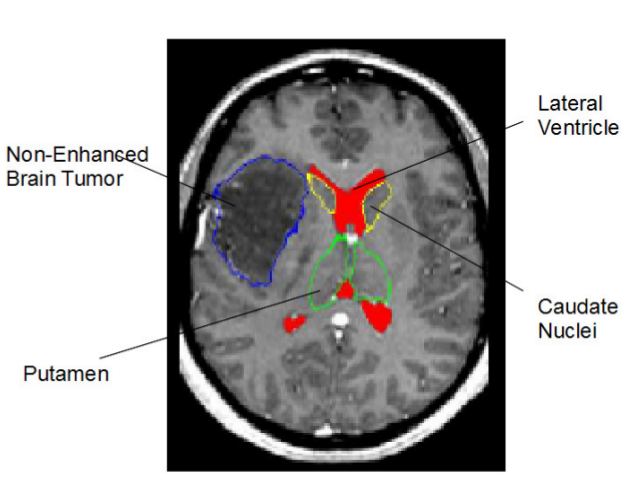
\includegraphics[width=.6\textwidth]{images/cerebrale.png}
% 	\caption{Extracted from .}
	\end{figure}
	\end{column}
\begin{column}{0.6\textwidth}
 \begin{itemize}
  \item An abnormal structure is present in the brain.
  \item A peripheral non-enhanced tumor is present in the right hemisphere.
 \end{itemize}
\end{column}
\end{columns}

\begin{columns}
\begin{column}{0.4\textwidth}
  \begin{figure}
  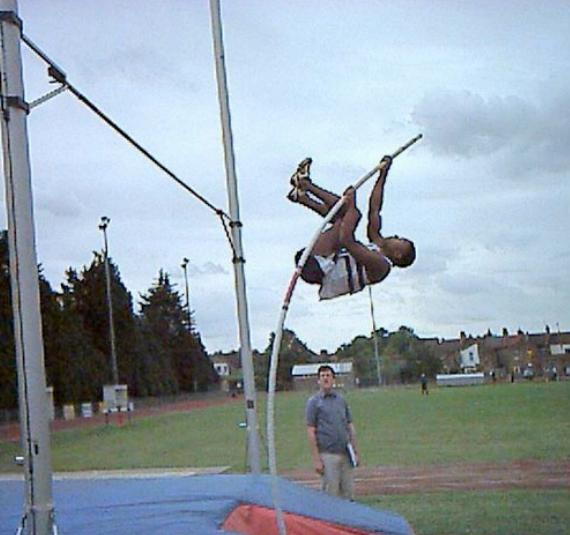
\includegraphics[width=.4\textwidth]{figures/highjump.png}
%   \caption{\tiny  Extracted from  .}
  \end{figure}
\end{column}

\begin{column}{0.6\textwidth}
 \begin{itemize}
  \item A person pulling a pole towards the ground.
  \item A middle phase of pole vaulting.
 \end{itemize}
\end{column}
\end{columns}

\begin{textblock}{100}(10,80)
\tiny 
[J. Atif \textit{et al.}, 2014] Explanatory reasoning for image understanding using formal concept analysis and description logics,	\emph{IEEE Transactions on Systems, Man and Cybernetics, 2014}.
\end{textblock}
\begin{textblock}{100}(10,85)
\tiny 
[S. Espinosa \textit{et al.}, 2007] Multimedia Interpretation as Abduction, \emph{20th International Workshop on Description Logics}.
\end{textblock}

\end{frame}

% \begin{frame}{note}
%   \begin{itemize}
%   \item This part we first give a concrete issue on brain imaging.
%   \item Three levels of understanding is given as the point of view of children, adult (certain level of education), expert doctor in brain analogy.
%   \item Translation from an image to a symbolic description
%   \item Therefore, the importance of structural knowledge representation, the importance of spatial relation, the importance of semantic gap difference between numeric representation and symbolic representation.
%  \end{itemize}
% \end{frame}
\begin{frame}{Related work}

 \begin{itemize}
  \item Graph-based approaches
  \begin{itemize}
   \item Bayesian network \textcolor{gray}{[S. Nikolopoulos \textit{et al.}, 2009]}.
   \item And-Or graph image grammar  \textcolor{gray}{[F. Han \textit{et al.}, 2009]} and \textcolor{gray}{[K. Tu \textit{et al.}, 2014]}.
  \end{itemize}
  \item Logic-based approaches
  \begin{itemize}
   \item Aggregation concepts (additional rules) \textcolor{gray}{[S. Espinosa \textit{et al.}, 2007]}.
   \item Knowledge representation based on formal concept analysis and reasoning based on morphological operators \textcolor{gray}{[J. Atif \textit{et al.}, 2014]}.
  \end{itemize}
 \end{itemize}
 
 \begin{alertblock}{Our goal}
   \begin{itemize}
    \item More expressive logic-based representation.
    \item Implicit information.
    \item Adaptive minimality criteria.
   \end{itemize}
 \end{alertblock}
\end{frame}



\begin{frame}{High level interpretation}
\begin{columns}
\begin{column}{0.6\textwidth}
 \begin{itemize}
  \item Computer aided diagnosis of a pathological brain image.
  \item Extraction of semantic descriptions from a given image in application terminology.
 \end{itemize}
\end{column}

\begin{column}{0.4\textwidth}
	\begin{figure}
	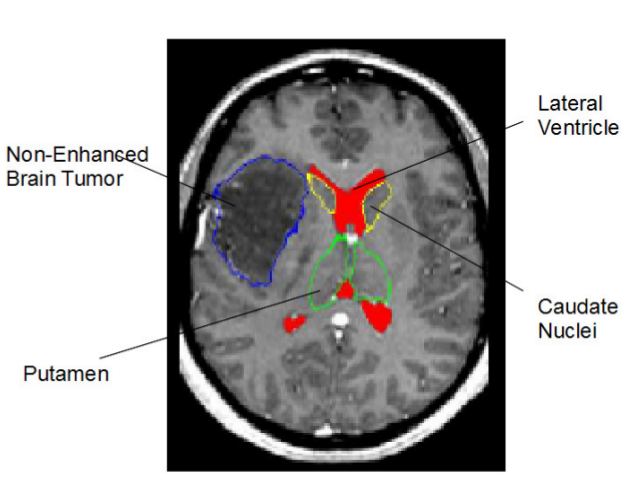
\includegraphics[width=\textwidth]{images/cerebrale.png}
	\end{figure}\vspace{-0.5cm}
	\end{column}
\end{columns}

\begin{block}{Components}
\centering
 \begin{itemize}
  \item Knowledge representation.
  \item Fuzzy representation.
  \item Qualitative spatial reasoning.
  \item Abductive reasoning.
 \end{itemize}
\end{block}

\end{frame}
% Image semantics is not inside the image.
% Image interpretation depends on a priori knowledge.
% => Use of explicit a priori knowledge for the interpretation.
% => Use of logic-based knowledge representation and reasoning framework.
% => Bridging the gap between logical representations and real data (in our
% case, image data) remains a challenging task and an open problem

% {Linearity}
\begin{frame}{General schema}
\begin{tikzpicture}
  \node (img1) {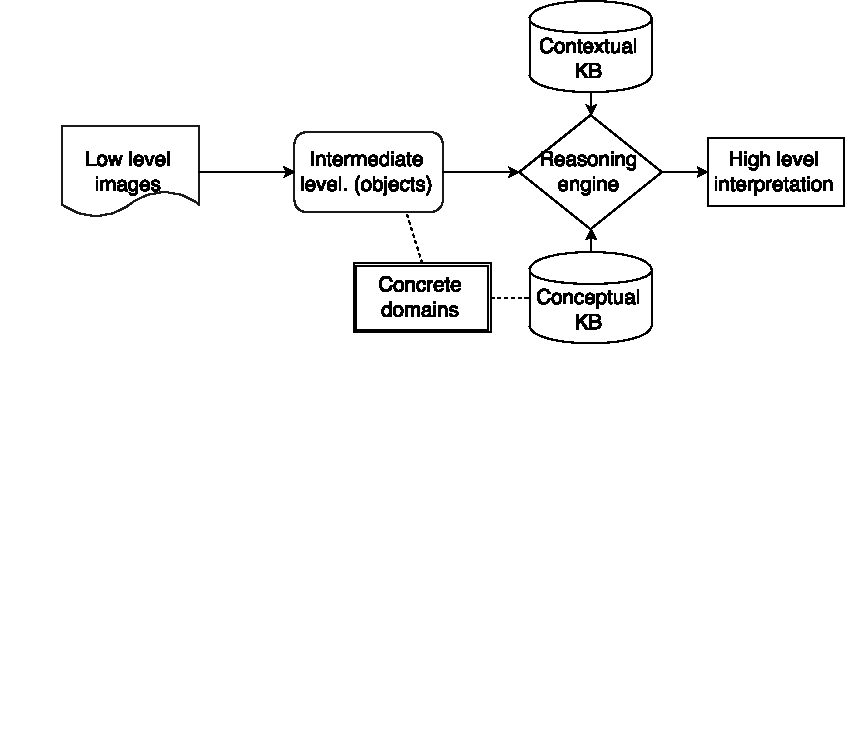
\includegraphics[width=0.95\linewidth,height=0.86\textheight]{images/general_schema_a_crop.pdf}};
  
  \onslide<2->{ \node (img2) {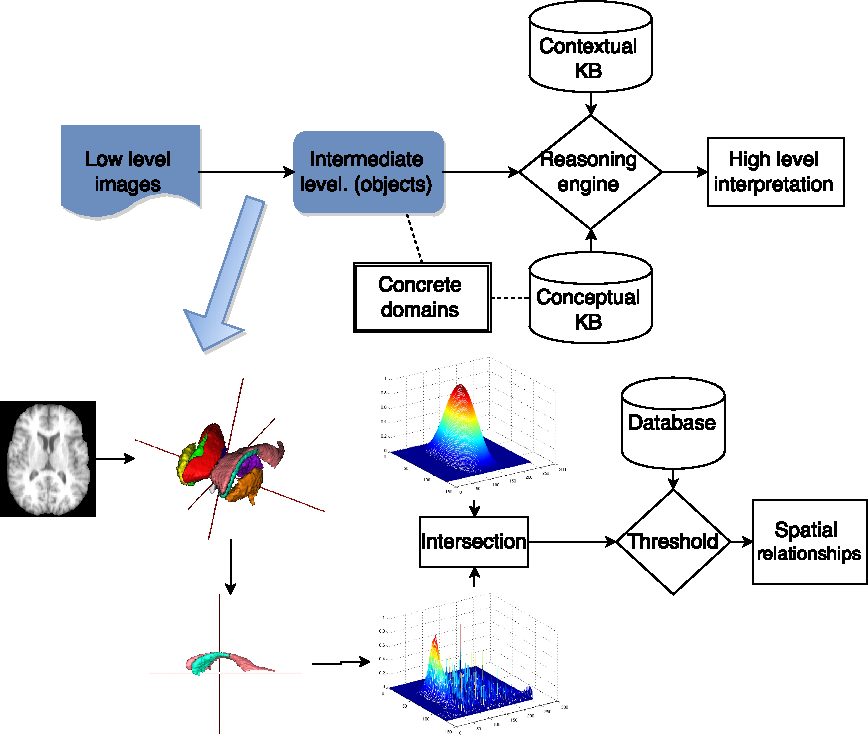
\includegraphics[width=0.95\linewidth,height=0.86\textheight]{images/general_schema_color_crop.pdf}}};
\end{tikzpicture}
\end{frame}
%====================Preliminary=================================
\section{Knowledge representation and reasoning}
\subsection{Conceptual knowledge representation}

\begin{frame}{Outline}
\begin{columns}
 \begin{column}{0.6\textwidth}
  \tableofcontents[currentsection,hideothersubsections,subsectionstyle=show/shaded]
 \end{column}

 \begin{column}{.4\textwidth}
  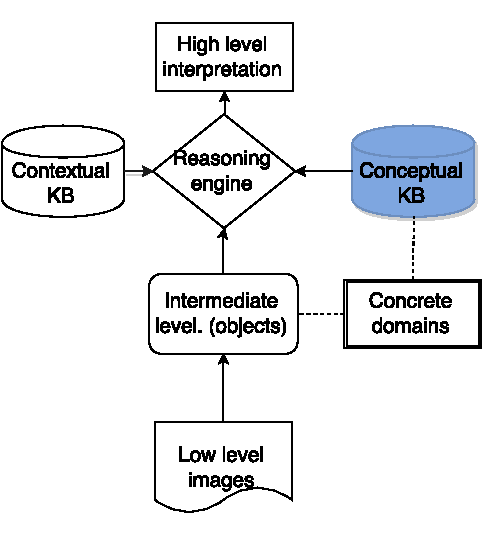
\includegraphics[width=.9\textwidth]{images/flowchart_kb_crop.pdf}
 \end{column}
\end{columns}
\end{frame}

\begin{frame}{Description Logics (Syntax)}
\begin{block}{Signature and constructors ($\mathcal{ALC}$)}
$Sig=(N_C,N_R,N_I)$: sets of concepts, roles and individuals.\\
$Con=\{\neg~(negation),\sqcap~(conjunction),\sqcup~(disjunction),$\\$~~~~~~~~~~\exists~(existential~restriction),\forall~(universal~restriction).\}$
\end{block}

\begin{exampleblock}{Examples}
\begin{enumerate}
 \item $BrainStructure \sqcap \exists (rightOf \sqcap closeTo). CNl$\\
 \item $\exists isPartOf. Brain \sqcap \neg BrainStructure$\\
 \item $LeftHemisphere\sqcup RightHemisphere$
\end{enumerate}
\end{exampleblock}
	\begin{figure}
	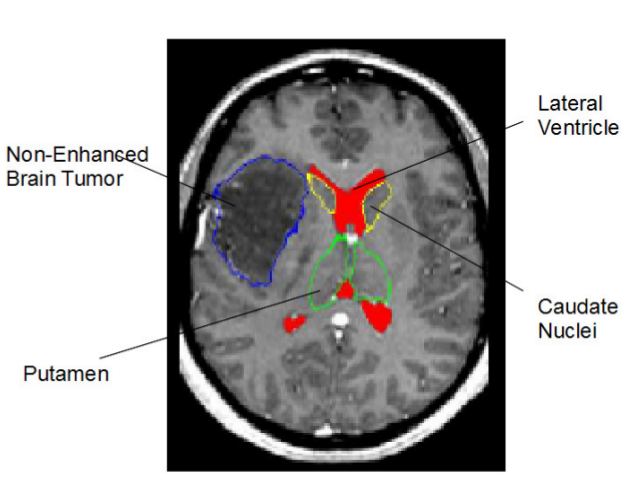
\includegraphics[width=.3\textwidth]{images/cerebrale.png}
	\end{figure}
\end{frame}

% Structural representation of knowledge (artificial language). Logic is clear without ambiguity.
%  Logic formalism, description logics. a formal language (syntax and semantics), structural representation, standard reasoning services. 
%  cite celine's paper, work of fma ontology.

\begin{frame}{Description Logics (Semantics)}
	\begin{block}{Semantics}
 An interpretation is a structure $\mathcal{I}=(\Delta^\mathcal{I},\cdot^\mathcal{I})$.
 \begin{itemize}
  \item $\Delta^\mathcal{I}$ is a domain (non-empty set).
   \item $\cdot^\mathcal{I}$ is a function that maps a concept to a subset of domain ($\Delta^\mathcal{I}$) and a role to a binary relation over the domain ($\Delta^\mathcal{I}\times \Delta^\mathcal{I}$).
 \end{itemize}
\end{block}

\begin{block}{Knowledge Base $\mathcal{K}$}
Terminological Box ($\mathcal{T}$) and Assertional Box ($\mathcal{A}$).
$\mathcal{K}=\{\mathcal{T},\mathcal{A}\}$
\begin{itemize}
 \item A set of general inclusion axioms ($C\sqsubseteq D$).
 \item A set of assertional facts ($a:C$, $\langle a,b\rangle: r$).
\end{itemize}

\end{block}
\end{frame}

\begin{frame}{Knowledge base example}
\begin{exampleblock}{Example}
\begin{columns}
 \begin{column}{0.6\textwidth}
 \centering
\scalebox{0.6}{\parbox{.5\linewidth}{%
\begin{align*}
 TBox=\{ Hemisphere &\sqsubseteq \exists isPartOf. Brain\\
	 BrainStructure &\sqsubseteq \exists isPartOf. Brain\\
	 BrainDisease &\sqsubseteq \exists isPartOf. Brain \sqcap \neg BrainStructure\\
	 Tumor  &\sqsubseteq BrainDisease\\
	 LVl &\sqsubseteq BrainStructure \sqcap \exists (rightOf \sqcap closeTo). CNl\\
	 LVr &\sqsubseteq BrainStructure \sqcap \exists (leftOf \sqcap closeTo). CNr\\
	 CNl &\sqsubseteq BrainStructure\\
	 CNr &\sqsubseteq BrainStructure\}\\
\end{align*}
}}
 \end{column}
\begin{column}{.4\textwidth}
Description of an expert's knowledge.
\end{column}
\end{columns}

\begin{columns}
 \begin{column}{0.6\textwidth}
 \centering
\scalebox{0.6}{\parbox{.5\linewidth}{%
\begin{align*}
 ABox=\{ a&: CNl \\
	 b&: Unknown~Object\\
	 c&: Brain \\
	 \langle a,b\rangle &: leftOf, closeTo \\
	 \langle b,c\rangle &: isPartOf\}
\end{align*}
}}
 \end{column}
 \begin{column}{.5\textwidth}
        Description of the observation.
  	\begin{figure}
	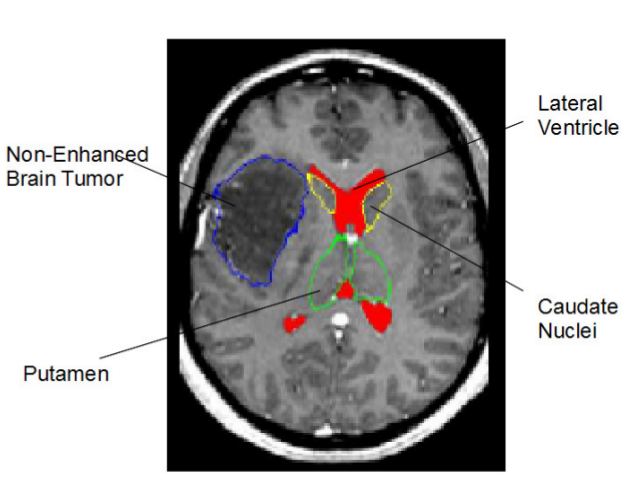
\includegraphics[width=.5\textwidth]{images/cerebrale.png}
	\end{figure}
 \end{column}
\end{columns}
\end{exampleblock}
\end{frame}

\subsection{Spatial representation and reasoning}
\begin{frame}{Outline}
\begin{columns}
 \begin{column}{0.6\textwidth}
  \tableofcontents[currentsection,hideothersubsections,subsectionstyle=show/shaded]
 \end{column}

 \begin{column}{.4\textwidth}
  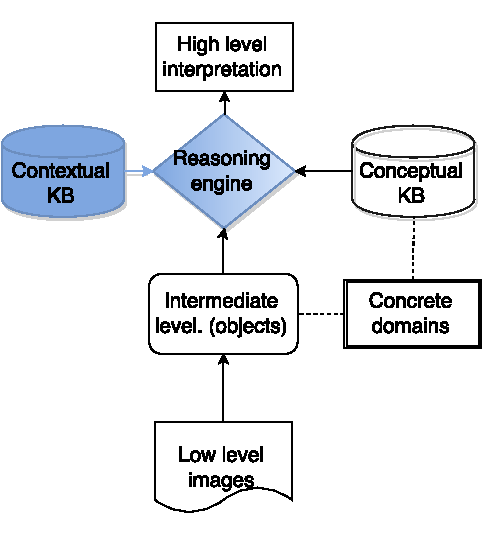
\includegraphics[width=.9\textwidth]{images/flowchart_sr_crop.pdf}
 \end{column}
\end{columns}
\end{frame}
\begin{frame}{Qualitative spatial representation (QSR)}
\begin{block}{Need for qualitative spatial reasoning}
\begin{itemize}
 \item Qualitative information in human expression.
 \item Reliable information in brain images.
\end{itemize}
\end{block}
\scalebox{0.6}{
	\begin{tabular}{|c|c|c|c|}
	\hline
	Constructor & Syntax & Semantics & Example\\
\hline
    Atomic role & $r$ & $r^\mathcal{I}\subseteq \Delta^\mathcal{I} \times \Delta^\mathcal{I}$ & $leftOf$\\
    Inverse role & $r^-$ & $\{(x,y),~x\in \Delta^\mathcal{I},~y\in \Delta^\mathcal{I} | ~(y,x)\in r^\mathcal{I}\}$ & $leftOf^-$ \\ 
    Role negation & $\neg r$ & $\Delta^\mathcal{I} \times \Delta^\mathcal{I} \setminus r^\mathcal{I}$ & $\neg leftOf$\\
    Role composition & $r_1\circ r_2$ & $\{(x,z), x\in \Delta^\mathcal{I},~z\in \Delta^\mathcal{I}| \exists y\in \Delta^\mathcal{I}, 
 (x,y)\in r_1^\mathcal{I}~and~(y,z)\in r_2^\mathcal{I}\}$ & $isPartOf\circ isPartOf$ \\
    Role conjunction & $r_1\sqcap r_2$ & $r_1^\mathcal{I} \cap r_2^\mathcal{I}$ & $leftOf\sqcap closeTo$\\
    Role disjunction & $r_1\sqcup r_2$ & $r_1^\mathcal{I} \cup r_2^\mathcal{I}$ & $closeTo\sqcup farFrom$\\
    Role inclusion & $r_1\sqsubseteq r_2$ &  $r_1^\mathcal{I} \subseteq r_2^\mathcal{I}$ & $adjacent\sqsubseteq closeTo$\\
    Role equivalence & $r_1\equiv r_2$ & $r_1^\mathcal{I} = r_2^\mathcal{I}$& $leftOf\equiv rightOf^-$\\
    \hline
	\end{tabular}}
\begin{exampleblock}{Proposition ($\mathcal{ALCHI_{R^+}}$)}
\begin{itemize}
 \item Inverse relation: $leftOf\equiv rightOf^-$, $hasPart\equiv isPartOf^-$
 \item Transitive relation: $isPartOf\circ isPartOf\sqsubseteq isPartOf$ 
 \item Symmetric relation: $closeTo\equiv closeTo^-$ 
\end{itemize} 
\end{exampleblock}
\end{frame}


\begin{frame}{Description Logics (Reasoning services)}
\begin{itemize}
\item Subsumption checking: $\mathcal{T}\vDash C\sqsubseteq D$ if $C^\mathcal{I}\subseteq D^\mathcal{I}$ for every model of $\mathcal{I}$ of $\mathcal{T}$.
\item Concept satisfiability: $C$ is satisfiable with respect to $\mathcal{T}$ if there exists a model $\mathcal{I}$ of $\mathcal{T}$ such that $C^\mathcal{I}\neq \emptyset$.
\end{itemize}
\begin{block}{}
 $$ \mathcal{T}\vDash C\sqsubseteq D~~iff~~\mathcal{T}\nvDash C\sqcap \neg D $$
\end{block}
\end{frame}


\begin{frame}{Illustration of QSR}
%  \begin{defn}[\textbf{Most specific concept} ]
% Given a TBox $\mathcal{T}$ and an associated interpretation $\mathcal{I}=(\Delta^{\mathcal{I}}, \cdot^{\mathcal{I}})$ in a DL $\mathcal{L}$,
% let $X\subseteq \Delta^{\mathcal{I}}$ be a subset of the interpretation space and $E$ a defined concept in $\mathfrak{C}(\mathcal{L})$. 
% The concept $E$ is defined as the most specific concept of $X$ w.r.t. $\mathcal{I}$ if:
% \begin{itemize}
%  \item $X \subseteq E^{\mathcal{I}}$.
%  \item for every defined concept $F\in\mathfrak{C}(\mathcal{L})$ with $X \subseteq F^{\mathcal{I}}$, we have $E \sqsubseteq_{\mathcal{T}} F$.
% \end{itemize}
% \label{def:msc}
% \end{defn}
% \cite{atif2014explanatory}
\begin{columns}
 \begin{column}{.5\textwidth}
   \centering
\scalebox{0.7}{\parbox{.5\linewidth}{%
\begin{align*}
 ABox=\{ a&: CNl \\
	 b&: Unknown~Object\\
	 c&: Brain \\
	 \langle a,b\rangle &: leftOf, closeTo \\
	 \langle b,c\rangle &: isPartOf\}
\end{align*}
}}
 \end{column}
 \begin{column}{.5\textwidth}
  	\begin{figure}
	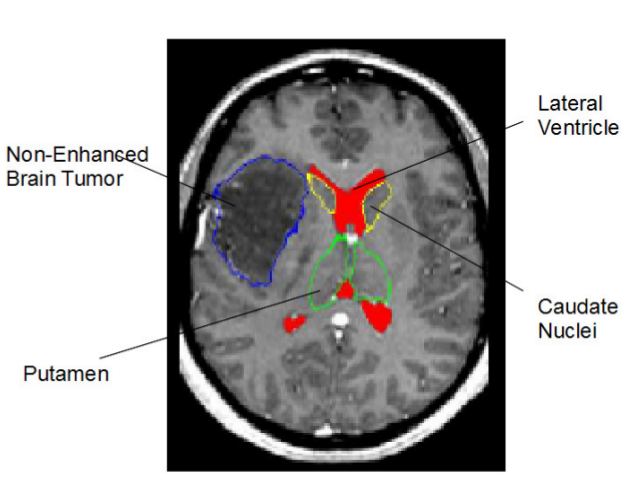
\includegraphics[width=.5\textwidth]{images/cerebrale.png}
	\end{figure}
 \end{column}
\end{columns}

\begin{exampleblock}{}
$$msc(b^\mathcal{I}):O\equiv \exists (leftOf^-\sqcap closeTo^-). CNl\sqcap \exists isPartOf.Brain$$
\end{exampleblock}
\begin{exampleblock}{}
$$H\equiv LVl\sqcap \exists isPartOf.Hemisphere$$
 $$ \mathcal{T}\vDash H\sqsubseteq O ~~iff~~ \mathcal{T}\nvDash H\sqcap \neg O $$
 $$LVl\sqcap \exists isPartOf.Hemisphere\sqcap( \forall (leftOf^-\sqcap closeTo^-).\neg CNl\sqcup \forall isPartOf.\neg Brain)$$
\end{exampleblock}


\end{frame}

\begin{frame}{Tableau method}
\scriptsize
\begin{block}{Tableau method}
\begin{itemize}
\item Starts from  $\mathcal{L}(x)=\{C\}$ with expansion rules to construct a model of $C$ where
  \begin{itemize}
  \item \scriptsize $x$ is an element of interpretation of the concept $C$ to test,
  \item $\mathcal{L}(x)$ is a set of concepts and $\mathcal{E}(\langle x,y\rangle)$ is  a set of roles. 
  \end{itemize}
\item Terminates when 
  \begin{itemize}
  \item \scriptsize a \textit{clash} occurs if $\{D,\neg D\}$ exists in a  $\mathcal{L}(\cdot)$,
  \item no rules can be applied.
  \end{itemize}
\end{itemize}
\end{block}


\begin{exampleblock}{Expansion rules}
\begin{itemize}
	 \item \scriptsize Conjunction
	       \begin{itemize}
	        \item  \scriptsize if $C_1\sqcap C_2\in \mathcal{L}(x)$ and if $\{C_1,C_2\}\nsubseteq \mathcal{L}(x)$, then $ \mathcal{L}(x)\rightarrow  \mathcal{L}(x)\cup \{C_1,C_2\}$.
	       \end{itemize}
% 	 \item Disjunction
% 	       \begin{itemize}\scriptsize
% 			\item  if $C_1\sqcup C_2\in \mathcal{L}(x)$ and if $\{C_1,C_2\} \cap \mathcal{L}(x)\neq \emptyset$, then $ \mathcal{L}(x)\rightarrow \mathcal{L}(x)\cup \{C\}~for ~some ~C\in\{C_1,C_2\}$.
% 	       \end{itemize}
	 \item \scriptsize Existential Quantification
	       \begin{itemize}\scriptsize
	       \item  \scriptsize if $\exists r.C\in \mathcal{L}(x)$ and $x$ has no successor $y$ with $C\notin \mathcal{L}(y)$, then create a new node $y$ with $\mathcal{E}(\langle x,y\rangle)$ and $\mathcal{L}(y)=\{C\}$
	       \end{itemize}
% 	 \item Universal Quantification
% 	       \begin{itemize}\scriptsize
%  	        \item   if $\forall r.C\in \mathcal{L}(x)$, if there exists an successor $y$ of $x$ with $C\notin \mathcal{L}(y)$, then $ \mathcal{L}(y)\rightarrow  \mathcal{L}(y)\cup \{C\}$.
% 	       \end{itemize}	

	 \item $\cdots$
\end{itemize}
\end{exampleblock}
\end{frame}


\begin{frame}{Tableau method (example)}
\begin{center}
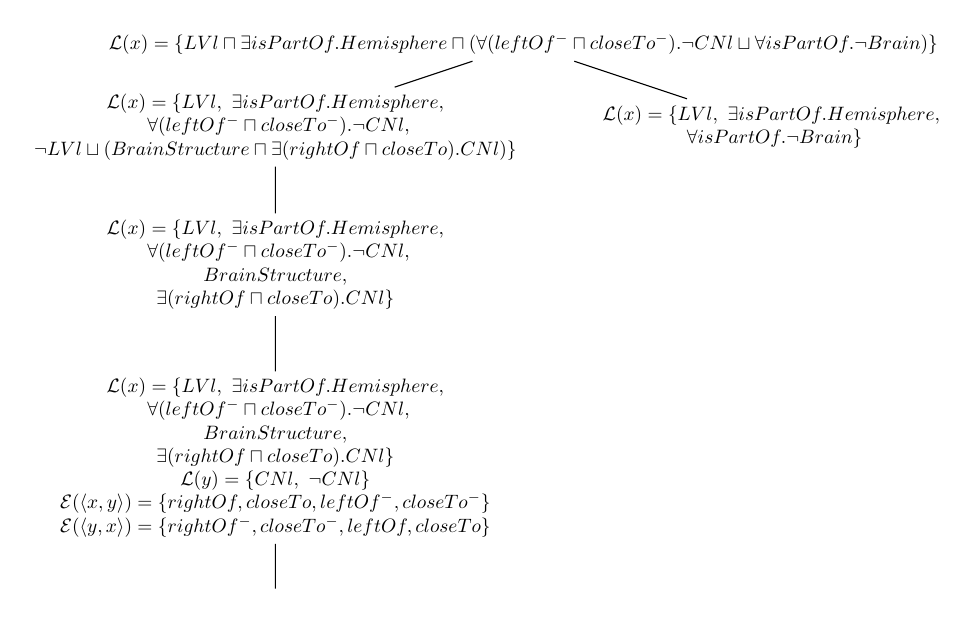
\begin{tikzpicture}[scale=0.7,transform shape,every text node part/.style={align=center},level 1/.style={level distance=1.5cm, sibling distance=9cm}, level 2/.style={level distance=2.5cm, sibling distance=6cm},
level 3/.style={level distance=3.5cm}, level 4/.style={level distance=2.5cm}]
\node [sibling distance=18cm] {$\mathcal{L}(x)=\{ LVl\sqcap \exists isPartOf.Hemisphere\sqcap (\forall (leftOf^-\sqcap closeTo^-).\neg CNl\sqcup \forall isPartOf.\neg Brain)\}$}
	      child{ node {$\mathcal{L}(x)=\{ LVl,~\exists isPartOf.Hemisphere,$\\$~\forall (leftOf^-\sqcap closeTo^-).\neg CNl,$\\$\neg LVl \sqcup (BrainStructure \sqcap \exists (rightOf \sqcap closeTo).CNl)\}$}
		            child{ node {$\mathcal{L}(x)=\{ LVl,~\exists isPartOf.Hemisphere,$\\$~\forall (leftOf^-\sqcap closeTo^-).\neg CNl,$\\$BrainStructure,$\\$\exists (rightOf \sqcap closeTo).CNl\}$}
				  child{ node {$\mathcal{L}(x)=\{ LVl,~\exists isPartOf.Hemisphere,$\\
				  $~\forall (leftOf^-\sqcap closeTo^-).\neg CNl,$\\$BrainStructure,$\\$\exists (rightOf \sqcap closeTo).CNl\}$\\
				  $\mathcal{L}(y)=\{CNl,~\neg CNl\}$\\
				  $\mathcal{E}(\langle x,y \rangle)=\{rightOf,closeTo,leftOf^-,closeTo^-\}$\\
				  $\mathcal{E}(\langle y,x\rangle)=\{rightOf^-,closeTo^-,leftOf,closeTo\}$}
				  child{ node{$\boxtimes$}}}}}
	      child{ node {$\mathcal{L}(x)=\{ LVl,~\exists isPartOf.Hemisphere,$\\$~\forall isPartOf.\neg Brain\}$}};
\end{tikzpicture}  
\end{center}
\end{frame}
%====================Ongoing work=================================
\section{Abductive reasoning}
\begin{frame}{Outline}
\begin{columns}
 \begin{column}{0.6\textwidth}
  \tableofcontents[currentsection,hideothersubsections,subsectionstyle=show/shaded]
 \end{column}

 \begin{column}{.4\textwidth}
  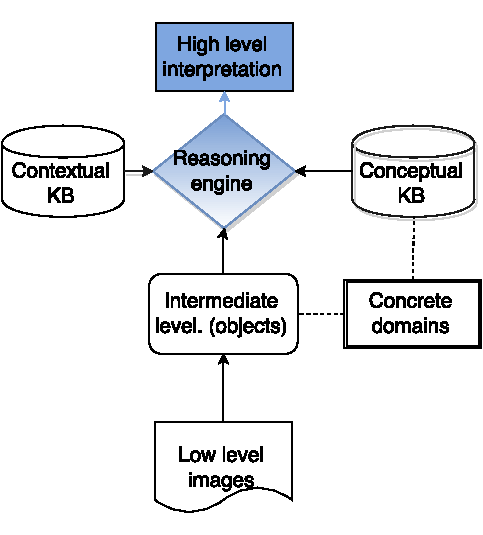
\includegraphics[width=.9\textwidth]{images/flowchart_ar_crop.pdf}
 \end{column}
\end{columns}
\end{frame}
\begin{frame}{Abductive reasoning}
%  from observation to explanation but whether it is necessary to present here or after.
%  Need of non-monotonic reasoning tools, i.e. image interpretation as an
% abduction problem :
% A scene is viewed as an observation and the task of interpretation is
% considered as the best explanation considering the knowledge about
% the scene context
\begin{itemize}
 \item Inference to the best explanation.
\end{itemize}
\begin{block}{Abductive reasoning for image interpretation}
 Given a knowledge base $\mathcal{K}$ and an observation concept $\mathcal{O}$, the  hypothesis $\mathcal{H}$ is an explanation of  $\mathcal{O}$ if  $$\mathcal{K}\vDash \mathcal{H}\sqsubseteq \mathcal{O}$$
\end{block}

\begin{block}{Satisfiability test}
$$\mathcal{K}\nvDash \mathcal{H}\sqcap \neg \mathcal{O}$$
\end{block}

\begin{exampleblock}{Strategy}
 $$\mathcal{H}\sqcap \neg\mathcal{O}~~(unsatisfiable?)$$ 
 
\end{exampleblock}
\end{frame}

\begin{frame}{An application example}
\begin{exampleblock}{}
\begin{columns}
 \begin{column}{0.6\textwidth}
 \centering
\scalebox{0.7}{\parbox{.5\linewidth}{%
\begin{align*}
\mathcal{T}=\{~SmallDeformingTumor &\sqsubseteq BrainTumor\\
 &\sqcap \exists hasEnhancement. NonEnhanced \\
&\sqcap \exists hasBehavior. Infiltrating  \\
PeripheralDeformingTumor &\sqsubseteq BrainTumor\\
& \sqcap \exists farFrom. LateralVentricle \\
& \sqcap \exists hasLocation. PeripheralCerebralHemisphere \} 
\end{align*}\vspace{-0.9cm}
% \tikzoverlay (n1) at (8cm,2cm) {%
\begin{align*}
\mathcal{O} =\{&~\exists hasEnhancement. NonEnhanced \\
 &\sqcap \exists farFrom. LateralVentricle \\
&\sqcap \exists hasLocation. PeripheralCerebralHemisphere \} 
\end{align*}
}} 
% };
 \end{column}
\begin{column}{.4\textwidth}
% \tikzoverlay (n2) at (5cm,0cm) {
  	\begin{figure}
	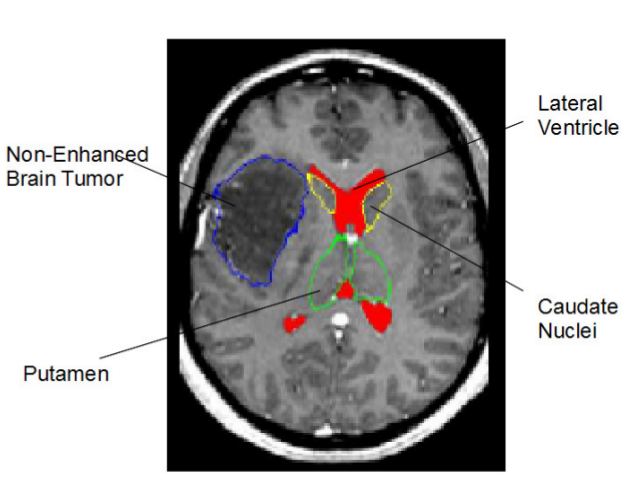
\includegraphics[width=.6\textwidth]{images/cerebrale.png}
	\end{figure}
% 	};
 \centering
%          \tikzoverlay (n3) at (5cm,0cm) {
\scalebox{0.7}{\parbox{.5\linewidth}{%
\begin{align*}
 ABox=\{ a&: CNl \\
	 b&: Unknown~Object\\
	 c&: Brain \\
	 \langle a,b\rangle &: leftOf, closeTo \\
	 \langle b,c\rangle &: isPartOf\}
\end{align*}
}}
% };

\end{column}
\end{columns}

% \begin{columns}
%  \begin{column}{0.6\textwidth}
% 
%  \end{column}
%  \begin{column}{.5\textwidth}
%         Description of the observation.
%   	\begin{figure}
% 	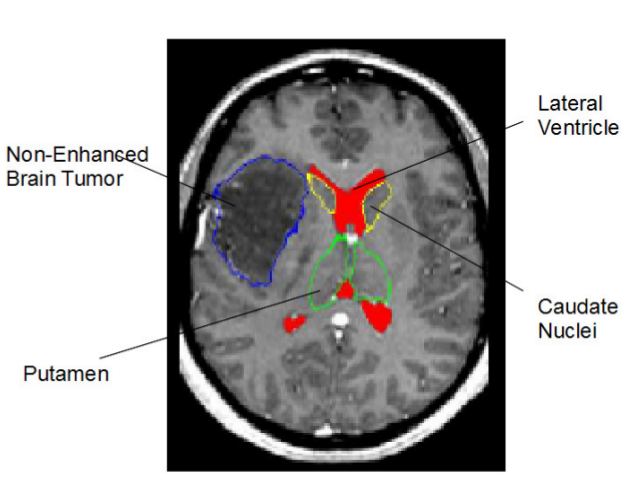
\includegraphics[width=.5\textwidth]{images/cerebrale.png}
% 	\end{figure}
%  \end{column}
% \end{columns}
\end{exampleblock}
% \begin{tikzpicture}[remember picture, overlay]
%   \path [line width=0.3cm,->] (n1.south) edge (n3.south);
%   \path [line width=0.3cm,->] (n3.north) edge (n2.south);
%   \path [line width=0.3cm,->] (n2.east) edge (n1.west);
% \end{tikzpicture}
%  
\end{frame}


\begin{frame}{Knowledge Integration}
\begin{defn}[Internalized concept]
Let $\mathcal{T}$ be a TBox and a set of axioms formulated as $C_i \sqsubseteq D_i$. The internalized concept of the TBox is defined as follows:
$$C_\mathcal{T} \equiv \sqcap_{(C_i \sqsubseteq D_i\in \mathcal{T})} (\neg C_i \sqcup D_i) $$
\label{def:ic}
\end{defn}
% ~\cite{baader2003description}
 \begin{align*}
 C_\mathcal{T}\sqcap  \neg\mathcal{O}= \{ &(\neg SDT \sqcup (BT \sqcap \exists hE. NE \sqcap \exists hB. In)) \sqcap \\
 &(\neg PDT \sqcup ( BT \sqcap \exists fF. LV \sqcap \exists hL. PCH)) \sqcap \\
 &(\forall hE. \neg NE \sqcup \forall fF. \neg LV \sqcup \forall hL.\neg PCH )\}
\end{align*}
\end{frame}







%  QSR is important, so it's the first step of our study.
%  presentation formally language we intend to use and proposed tableau reasoning.

% In the reference, topological relation is intensively studied,
% However, the metric relations are important in our context, in other reference , the space is divided into subparts and the object is regarded as a point (often the gravity point),
% This kind of representation is not accurate and the transitivity is not guaranteed considering the form.

\begin{frame}{Generating potential hypotheses}
Six branches are open in the tableau at the end. In each one, the set of concepts that cannot be decomposed are:
 \begin{align*}
  H_1&=\{ SDT, PDT, \exists hE.NE\}\\
  H_2&=\{ SDT, PDT, \exists fF.LV\}\\
  H_3&=\{ SDT, PDT, \exists hL.PCH\}\\
  H_4&=\{ SDT, \neg BT, \forall fF. \neg LV, \forall hL. \neg PCH, \exists hE.NE\}\\
  H_5&=\{ PDT, \neg BT, \forall hE. \neg NE, \forall hB. \neg In, \exists fF.LV\}\\
  H_6&=\{ PDT, \neg BT, \forall hE. \neg NE, \forall hB. \neg In, \exists hL.PCH\}\\
 \end{align*}
 
 \begin{block}{Minimal hitting set (\textit{Complexity: NP-Complete.})} 
 \begin{center}
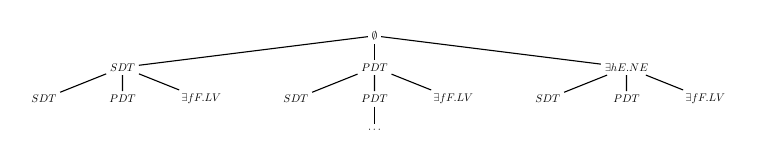
\begin{tikzpicture}[scale=0.4, transform shape, every text node part/.style={align=center},level 1/.style={level distance=1cm,sibling distance=8cm},level 2/.style={level distance=1cm, sibling distance=2.5cm}]
\node [sibling distance=12cm] {$\emptyset$}
child { node []{$SDT$}
     child{ node []{$SDT$}}
     child{ node []{$PDT$}}
     child{ node []{$\exists fF.LV$}}
}
child { node  []{$PDT$}
     child{ node []{$SDT$}}     
     child{ node []{$PDT$}
	child{ node []{$\cdots$}}}
     child{ node []{$\exists fF.LV$}}
}
child { node  []{$\exists hE.NE$}
     child{ node []{$SDT$}}     
     child{ node []{$PDT$}}
     child{ node []{$\exists fF.LV$}}
};
\end{tikzpicture}
\end{center}
 \end{block}
\end{frame}

\begin{frame}{Minimality criteria}
%  One potential hypothesis is the combination of these concepts using Algorithm \ref{algo:exhaustive}.
\begin{block}{Selecting the preferred explanation}
\begin{itemize}
  \item Consistency: $\mathcal{K}\cup H$ is consistent.  e.g. $SDT \sqcap \neg BT$, $PDT \sqcap \forall fF \neg LV$.
  \item Relevance: $\mathcal{O}$ is not entailed by $H$ ($H\nvDash \mathcal{O}$). e.g. irrelevant hypothesis: $\exists hE. NE \sqcap \exists fF. LV \sqcap \exists hL.PCH $
  \item Semantic minimality: $\nexists$ $H_i$ such that $H_i\vDash H$.\\
  For an abduction problem $\mathcal{P}=\langle \mathcal{T},\mathcal{H}, \mathcal{O}\rangle$, and $\{\langle P_{1},\dots,P_{n}\rangle\}$ potential hypotheses,
\begin{itemize}
\item  $P_{i}$ is a $\sqsubseteq -minimal$ explanation if there does not exist an explanation $P_{j}$ for $\mathcal{P}$ such that $P_{i}\sqsubseteq P_{j}$.
\end{itemize}
 \end{itemize}
\end{block}

% According to the subsumption criterion, $SDT \sqcap \exists fF.LV \sqcap \exists hL.PCH$
% and $PDT \sqcap \exists hE.NE$ are considered as preferred explanations. For example, 
% $SDT \sqcap PDT$ is subsumed by these two hypotheses. 
\begin{exampleblock}{Explanations}
 \begin{itemize}
 \item $PeripheralDeformingTumor \sqcap \exists hasEnhancement. NonEnhanced$
 \item $SmallDeformingTumor\sqcap \exists farFrom. LateralVentricle $\\ $\sqcap \exists hasLocation. PeripheralCerebralHemisphere$
\end{itemize}
\end{exampleblock}
\end{frame}


\section{Conclusion and perspectives}
\begin{frame}{Conclusions and perspectives}
% low level processing manipulation in image domain
% high level processing abduction
% 
% perspective more interaction between these two layers
\begin{columns}
 \begin{column}{.7\textwidth}
  
\begin{block}{Conclusion}
 \begin{itemize}
  \item A complete image interpretation system.
  \item A more expressive Description Logic language.
  \item An adaptive tableau method for image interpretation.
 \end{itemize}
\end{block}

\begin{block}{Perspectives}
\begin{itemize}
 \item Abductive reasoning:
 \begin{itemize}
  \item adding iteratively internalized concepts of corresponding axioms,
  \item assigning importance values for different levels of concepts.
 \end{itemize}
 \item Concrete domains (Connection between image and logic).
 \item Fuzzy representation.
\end{itemize}
\end{block}
 \end{column}

  \begin{column}{.3\textwidth}
    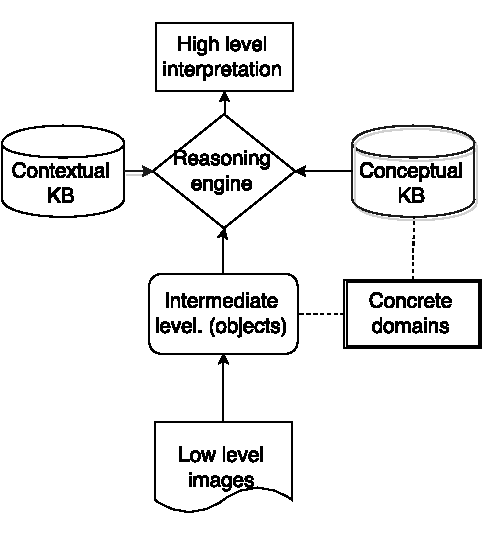
\includegraphics[width=.9\textwidth, height=.6\textheight]{images/flowchart_cp_crop.pdf}
  \end{column}


\end{columns}
\end{frame}


\begin{frame}{Q $\&$ A}
\begin{center}
 Thank you\\

Questions?
\end{center}
\end{frame}

%% Extra frames
\begin{frame}{Extra tableau}
\begin{center}
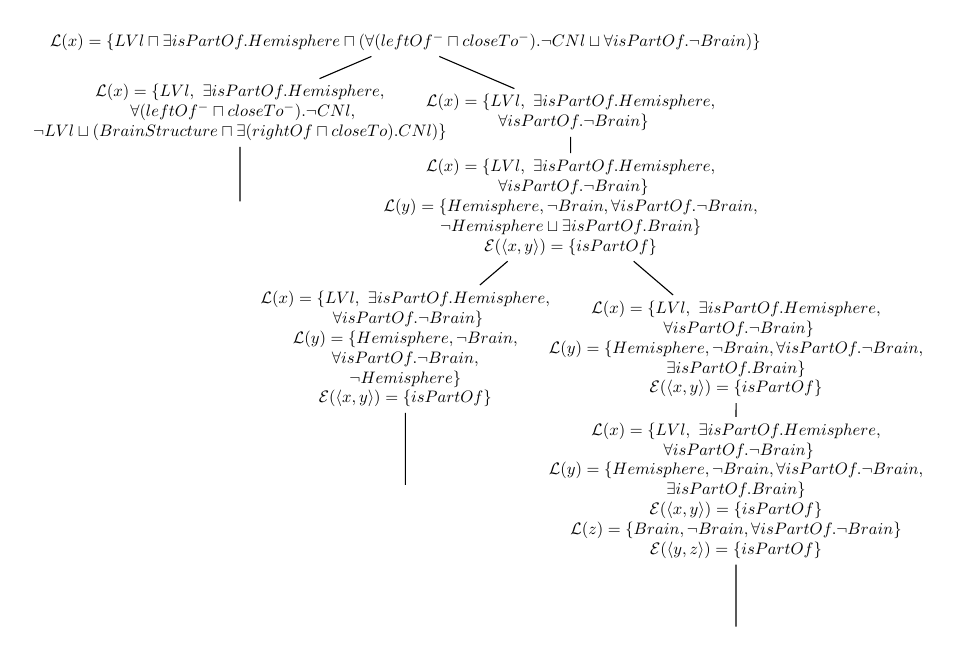
\begin{tikzpicture}[scale=0.6,transform shape,every text node part/.style={align=center},level 1/.style={level distance=1.5cm, sibling distance=7cm}, level 2/.style={level distance=2cm, sibling distance=6cm},
level 3/.style={level distance=3cm, sibling distance=7cm}]
\node [sibling distance=18cm] {$\mathcal{L}(x)=\{ LVl\sqcap \exists isPartOf.Hemisphere\sqcap ( \forall (leftOf^-\sqcap closeTo^-).\neg CNl\sqcup \forall isPartOf.\neg Brain)\}$}
	      child{ node {$\mathcal{L}(x)=\{ LVl,~\exists isPartOf.Hemisphere,$\\$~\forall (leftOf^-\sqcap closeTo^-).\neg CNl,$\\$\neg LVl \sqcup( BrainStructure \sqcap \exists (rightOf \sqcap closeTo).CNl)\}$}
				  child{ node{$\boxtimes$}}}
	      child{ node {$\mathcal{L}(x)=\{ LVl,~\exists isPartOf.Hemisphere,$\\$~\forall isPartOf.\neg Brain\}$}
		     child{ node{$\mathcal{L}(x)=\{ LVl,~\exists isPartOf.Hemisphere,$\\$~\forall isPartOf.\neg Brain\}$\\
				  $\mathcal{L}(y)=\{ Hemisphere, \neg Brain, \forall isPartOf. \neg Brain,$\\
				  $\neg Hemisphere \sqcup \exists isPartOf.Brain\}$\\
				  $\mathcal{E}(\langle x,y \rangle)=\{isPartOf\}$}
				  child{ node{$\mathcal{L}(x)=\{ LVl,~\exists isPartOf.Hemisphere,$\\$~\forall isPartOf.\neg Brain\}$\\
					      $\mathcal{L}(y)=\{ Hemisphere, \neg Brain,$\\$ \forall isPartOf. \neg Brain,$\\
					      $\neg Hemisphere\}$\\
					      $\mathcal{E}(\langle x,y \rangle)=\{isPartOf\}$ }
					      child{ node{$\boxtimes$}}}
				  child{ node{$\mathcal{L}(x)=\{ LVl,~\exists isPartOf.Hemisphere,$\\$~\forall isPartOf.\neg Brain\}$\\
					      $\mathcal{L}(y)=\{ Hemisphere, \neg Brain, \forall isPartOf. \neg Brain$,\\
					      $ \exists isPartOf.Brain\}$\\
					      $\mathcal{E}(\langle x,y \rangle)=\{isPartOf\}$ }
					child{ node{$\mathcal{L}(x)=\{ LVl,~\exists isPartOf.Hemisphere,$\\$~\forall isPartOf.\neg Brain\}$\\
						    $\mathcal{L}(y)=\{ Hemisphere, \neg Brain, \forall isPartOf. \neg Brain$,\\
						    $ \exists isPartOf.Brain\}$\\
						    $\mathcal{E}(\langle x,y \rangle)=\{isPartOf\}$\\
						    $\mathcal{L}(z)=\{Brain,\neg Brain,\forall isPartOf.\neg Brain\}$\\
						    $\mathcal{E}(\langle y,z\rangle)=\{isPartOf\}$}
						    child{ node{$\boxtimes$}}}}}};
\end{tikzpicture}  
\end{center}
\end{frame}
\end{document}
